\section{Vulnerability Database}
\sectionframe

\begin{frame}[fragile]
\frametitle{Greenbone Database}
\begin{columns}[T,totalwidth=\textwidth]
\begin{column}{0.75\textwidth}
The Database is the core of OpenVAS.\\
It contains all the information about the vulnerabilities
and the way to check them.\\
\begin{tabular}{|c|c|}
    \hline
    \textbf{Type of Feed} & \textbf{Price} \\
    \hline
    Greenbone Community Feed & Free \\
    \hline
    Greenbone Security Feed & 2524 €/year \\
    \hline
\end{tabular}


\includegraphics[width=0.75\textwidth]{images/GSF.png}
\end{column}
\begin{column}{0.25\textwidth}

\begin{figure}
\begin{center}

\includegraphics[height=0.4\textheight]{images/postgesql.png}
\end{center}
\end{figure}
\end{column}
\end{columns}
\end{frame}

\begin{frame}[fragile]
    \frametitle{Database's Structure}
    \begin{columns}[T,totalwidth=\textwidth]
    \begin{column}{0.33\textwidth}
        \begin{center}
        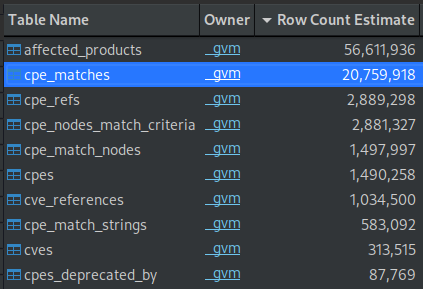
\includegraphics[width=0.95\textwidth]{images/db1.png}\\[50pt]
        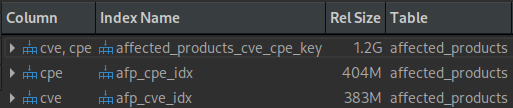
\includegraphics[width=0.95\textwidth]{images/db3.png}
        \end{center}
    \end{column}
    \begin{column}{0.34\textwidth}
        %\begin{center}
        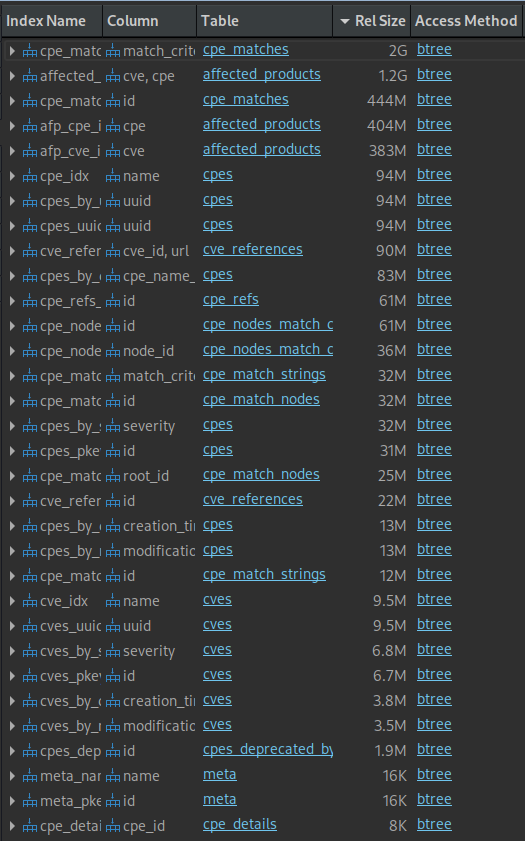
\includegraphics[width=1.0\textwidth]{images/db5.png}
        %\end{center}
    \end{column}
    \begin{column}{0.33\textwidth}
        \begin{center}
        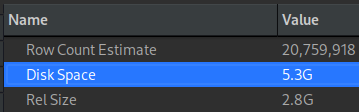
\includegraphics[width=0.95\textwidth]{images/db4.png}\\[70pt]
        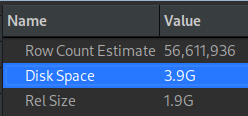
\includegraphics[width=0.95\textwidth]{images/db2.png}
        \end{center}
    \end{column}
    \end{columns}
\end{frame}

\begin{frame}[fragile]
    \frametitle{Feed Update}
    \begin{columns}[T,totalwidth=\textwidth]
    \begin{column}{0.5\textwidth}
    %    \begin{center}
        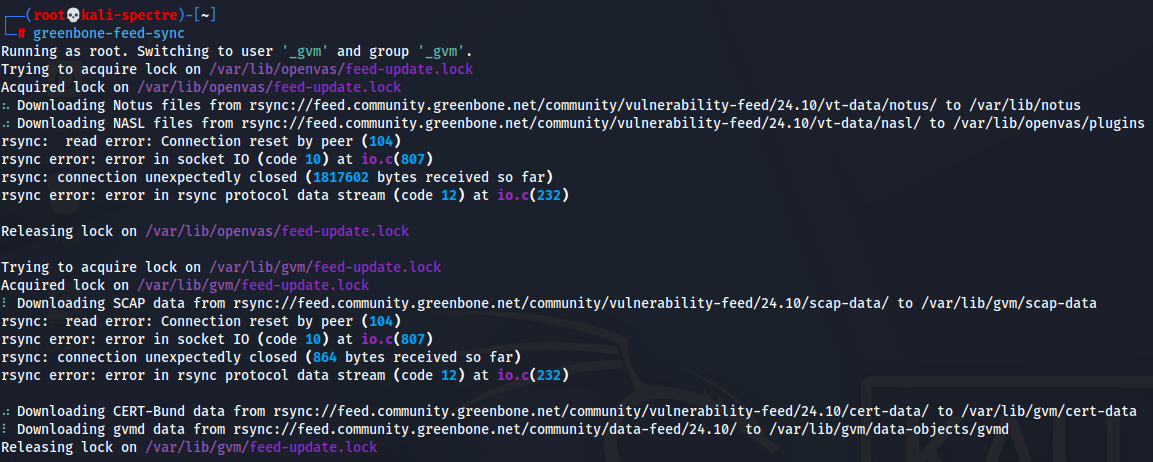
\includegraphics[width=0.95\textwidth]{images/screen_gvm1.png}\\
        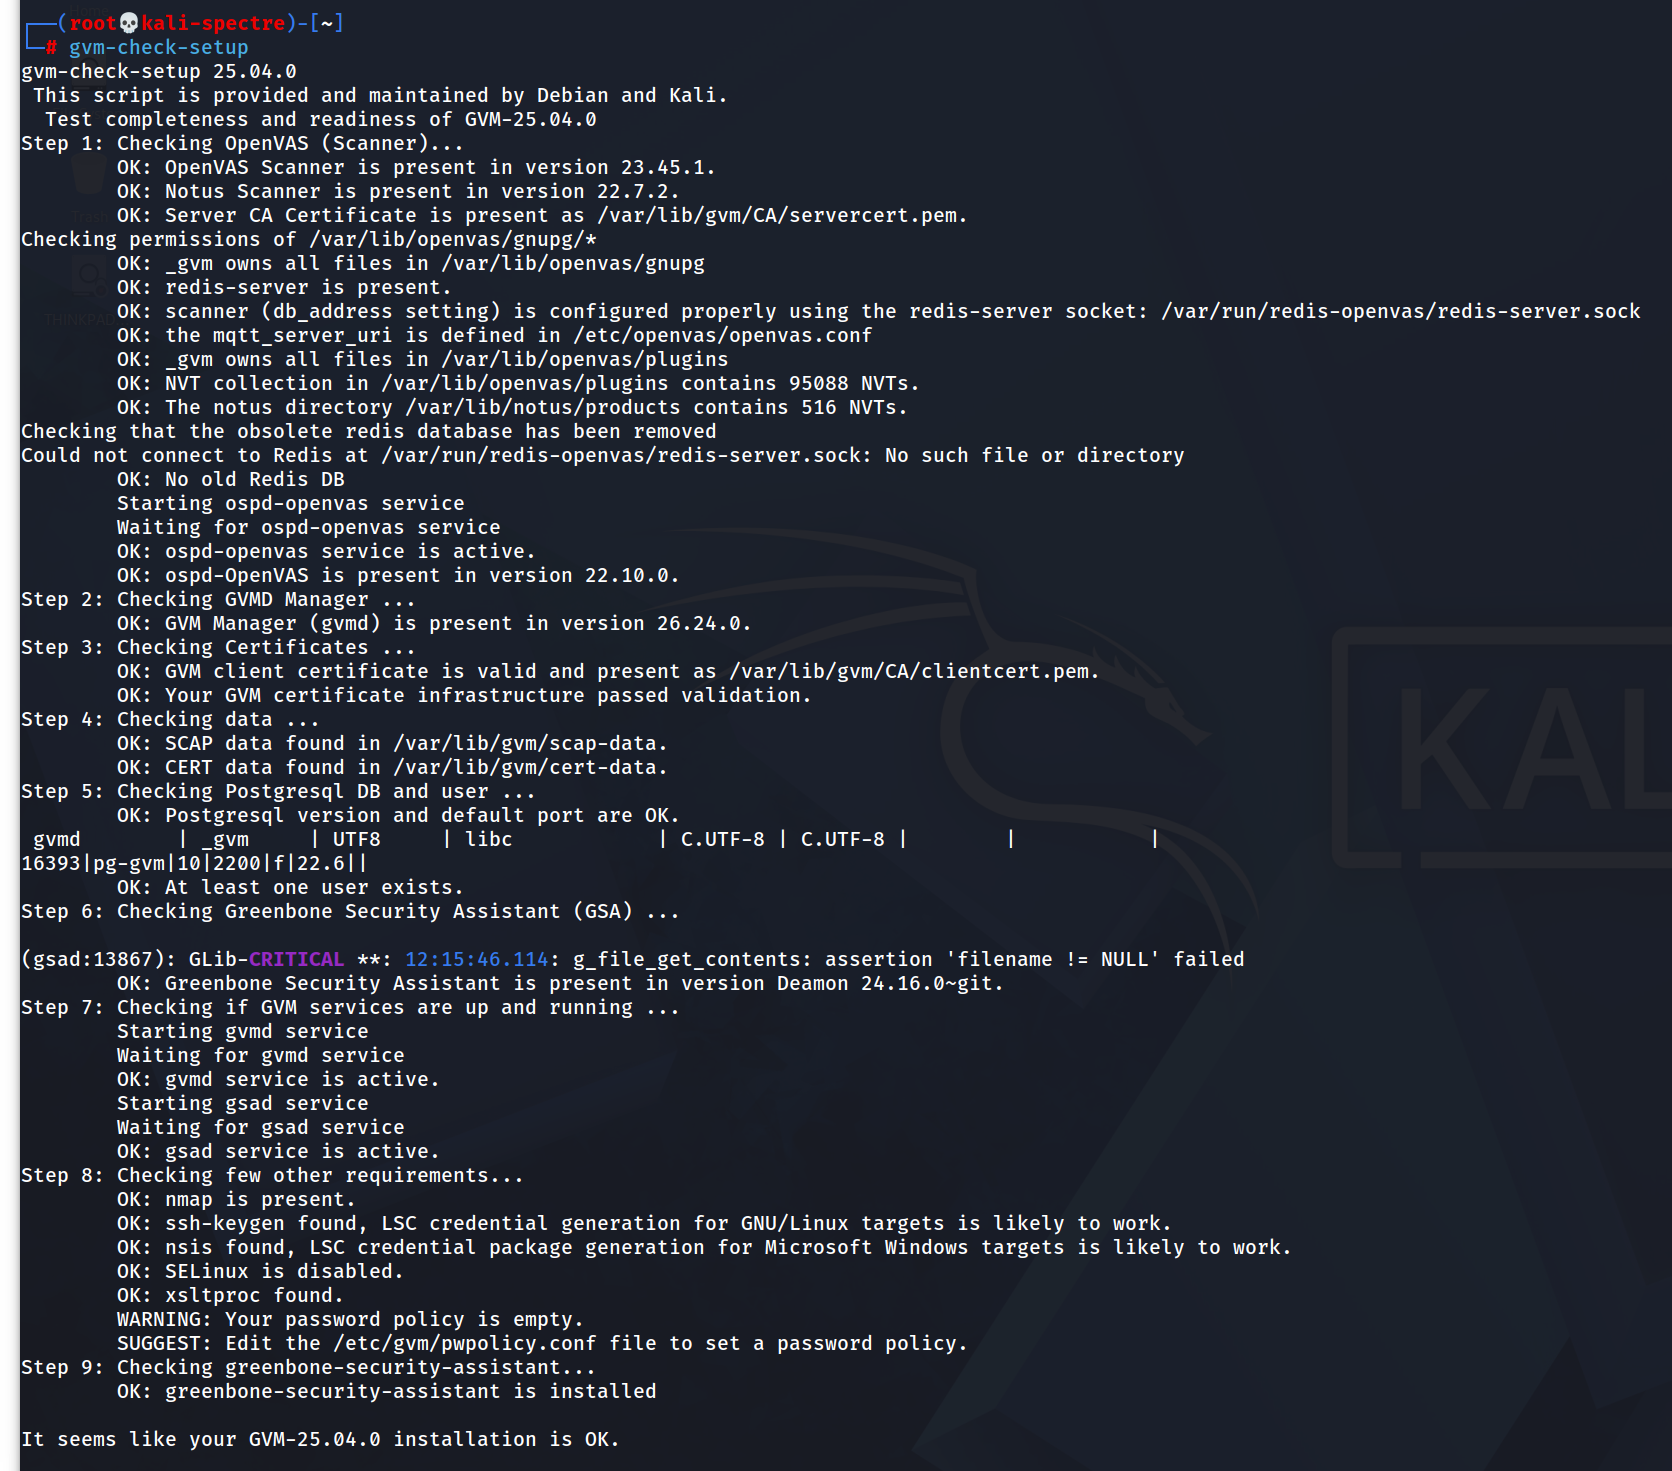
\includegraphics[width=0.7\textwidth]{images/screen_gvm2.png}
    %    \end{center}
    \end{column}
    \begin{column}{0.5\textwidth}
    %    \begin{center}
        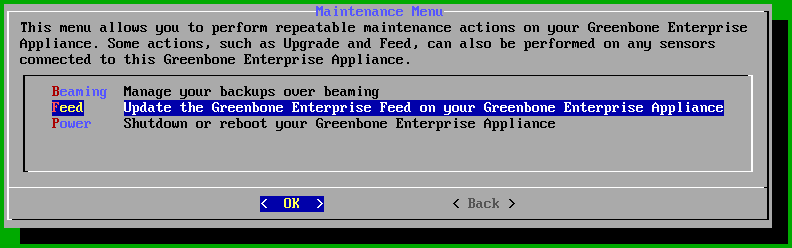
\includegraphics[width=0.9\textwidth]{images/gs_feed_update.png}\\[4pt]
        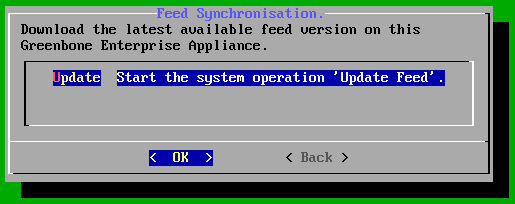
\includegraphics[width=0.9\textwidth]{images/gs_feed_update2.png}\\[4pt]
        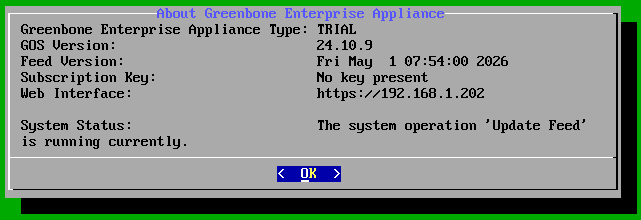
\includegraphics[width=0.9\textwidth]{images/gs_info.png}
    %    \end{center}
    \end{column}    
    \end{columns}
\end{frame}

\begin{frame}[fragile]
    \frametitle{Feed Status}
    \begin{center}
        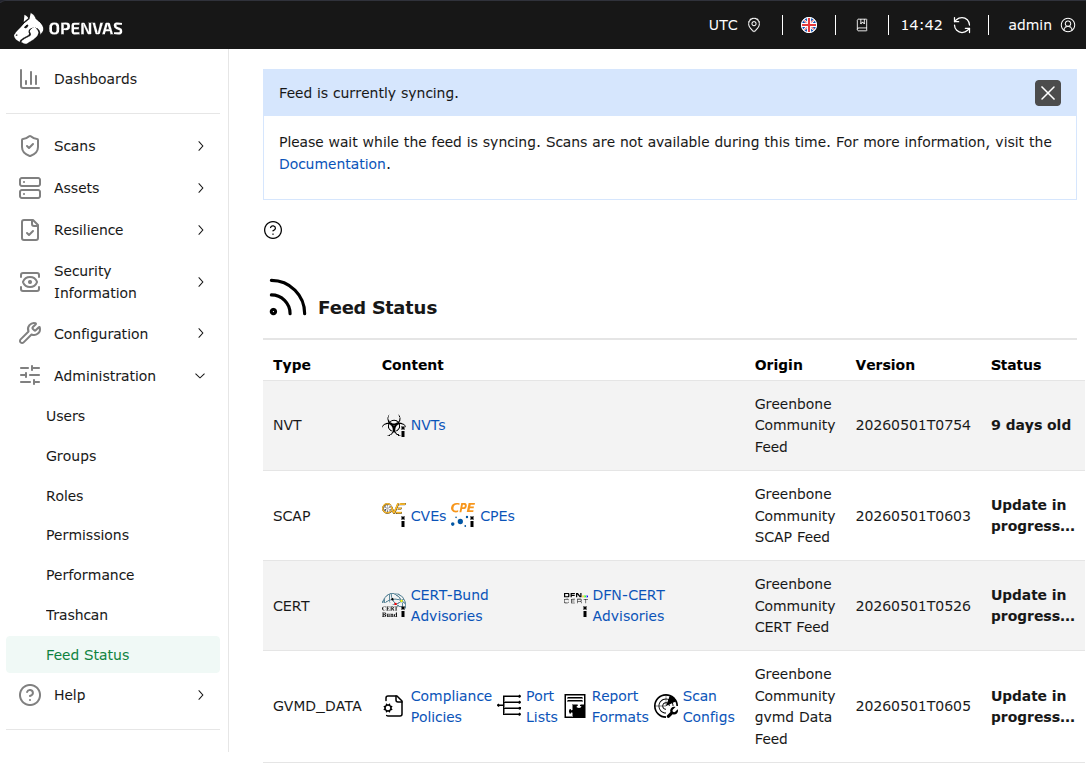
\includegraphics[height=0.75\textheight]{images/gs_feed_status.png}
    \end{center}
\end{frame}
